\begin{figure}[htp!]
    \centering

    \begin{subfigure}[t]{0.45\textwidth}
        \centering
        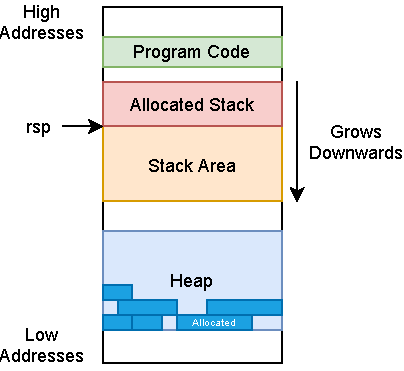
\includegraphics[height=5.5cm]{assets/figures/chapter2/memory-layout.pdf}
        \caption{Process memory layout}
        \label{subfig:memory:memory-layout}
    \end{subfigure}
    \begin{subfigure}[t]{0.45\textwidth}
        \centering
        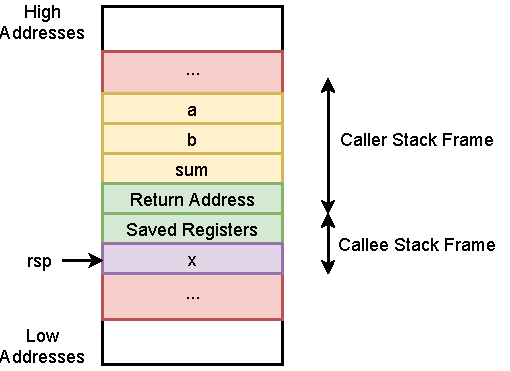
\includegraphics[height=5.5cm]{assets/figures/chapter2/stack-frame.pdf}
        \caption{Stack frame layout for function \textit{add} in Listing~\ref{lst:stack-example-function}}
        \label{subfig:memory:stack-frame}
    \end{subfigure}

    \caption{Go memory and stack frame layout}
    \label{fig:memory-stack}
\end{figure}
